\documentclass{article}
\usepackage{amsmath}

\usepackage[margin=1in]{geometry}
\usepackage{listings}
\usepackage{xcolor}
\usepackage{graphicx}

\lstset{
  basicstyle=\ttfamily,
  columns=fullflexible,
  breaklines=true,
  postbreak=\mbox{\textcolor{red}{$\hookrightarrow$}\space},
  frame=single,
  language=Matlab
}

\begin{document}

\section*{For Transfer Function 1: \( G(s) = \frac{K}{s(s+2)(s+4)(s+10)} \)}

\begin{enumerate}
    \item \textbf{Poles and Zeros:}
    \begin{itemize}
        \item Poles: \( 0, -2, -4, -10 \)
        \item Zeros: None
    \end{itemize}

    \item \textbf{Asymptotes:}
    \begin{itemize}
        \item Number of Asymptotes: \( n - m = 4 - 0 = 4 \) (where \( n \) is number of poles and \( m \) is number of zeros)
        \item Angles of Asymptotes: \( \theta = \frac{(2k+1)180^\circ}{n-m} \) for \( k = 0, 1, 2, 3 \)
        \begin{itemize}
            \item For \( k = 0 \): \( \theta = 45^\circ \)
            \item For \( k = 1 \): \( \theta = 135^\circ \)
            \item For \( k = 2 \): \( \theta = 225^\circ \)
            \item For \( k = 3 \): \( \theta = 315^\circ \)
        \end{itemize}
        \item Intersection with Real Axis: \( \sigma = \frac{\sum \text{poles} - \sum \text{zeros}}{n - m} = \frac{0 - 2 - 4 - 10}{4} = -4 \)
    \end{itemize}

    \item \textbf{Break Away/Break-In Points:}

The characteristic equation is \( 1 + KG(s) = 0 \) or \( s(s+2)(s+4)(s+10) + K = 0 \).

First, rearrange the equation to express \( K \) as a function of \( s \):
\[ K = -s(s+2)(s+4)(s+10) \]

Now, differentiate both sides of this equation with respect to \( s \):
\begin{align*}
\frac{dK}{ds} &= \frac{d}{ds} \left[ -s(s+2)(s+4)(s+10) \right] \\
&= -\left[ (s+2)(s+4)(s+10) + s(s+4)(s+10) + s(s+2)(s+10) + s(s+2)(s+4)\right] \\
&= 4s^3+48s^2+136s+80
\end{align*}


    \item \textbf{Departure and Arrival Angles:}
    \begin{itemize}
        \item Since there are no zeros, there are no arrival angles.
        \item Departure angles are not applicable as all poles are real.
    \end{itemize}
    \item \textbf{Finding angle of damping factor:}
    
In control system analysis, the damping factor \( \zeta \) characterizes a system's transient response. It is defined for a second-order system as:
\[ \zeta = \frac{-\sigma}{\sqrt{\sigma^2 + \omega_n^2}} \]
where \( \sigma \) is the pole's real part, and \( \omega_n \) is the natural frequency.

A damping factor of \( \zeta = \sqrt{2}/2 \) or about \( 0.707 \) signifies a critically damped system, marking the boundary between underdamped and overdamped states. This condition implies that the system's poles in the complex plane form a \( 45^\circ \) angle with the negative real axis. The angle \( \theta \), derived from the pole's position in the s-plane, is calculated as:
\[ \theta = \tan^{-1}\left(\frac{\text{Imaginary part of pole}}{\text{Real part of pole}}\right) = \tan^{-1}(1) = 45^\circ \]

Therefore, a \( 0.707 \) damping factor corresponds to pole angles of \( 45^\circ \) in the s-plane, indicative of a critically damped system.

        
    \item \textbf{Root Locus Plot:}
    \newline
    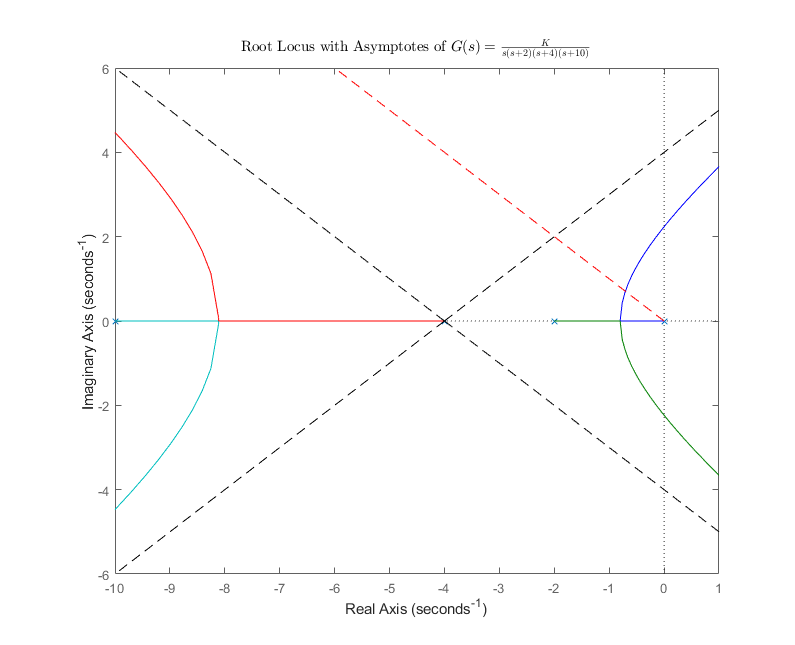
\includegraphics[width=0.9\textwidth]{7-16A.png}
\begin{lstlisting}[caption={MATLAB Code to Plot Root Locus of \( G(s) \)}]
% Define the zeros, poles, and gain of the transfer function
zeros = [];
poles = [0, -2, -4, -10];
gain = 1;

% Create the transfer function
G = zpk(zeros, poles, gain);

% Plot the root locus
figure;
rlocus(G);
hold on;

% Calculate the centroid of the asymptotes
centroid = (sum(poles) - sum(zeros)) / (length(poles) - length(zeros));

% Calculate and plot the asymptotes
n_asymptotes = length(poles) - length(zeros);
for k = 0:n_asymptotes-1
    angle = ((2*k + 1) * pi) / n_asymptotes;
    x = centroid + 1000 * cos(angle);
    y = 1000 * sin(angle);
    plot([centroid, x], [0, y], '--k'); % dashed line for asymptotes
end

% Plot the 135-degree line
angle_135 = 3*pi/4; % 135 degrees in radians
x_135 = 1000 * cos(angle_135);
y_135 = 1000 * sin(angle_135);
plot([0, x_135], [0, y_135], '--r'); % red dashed line for 135-degree angle

% Setting the title and labels
title('Root Locus with Asymptotes of $G(s) = \frac{K}{s(s+2)(s+4)(s+10)}$', 'Interpreter', 'latex');
xlabel('Real Axis');
ylabel('Imaginary Axis');
ylim([-6 6])
xlim([-10 1])
hold off;
\end{lstlisting}
\item \textbf{Finding K:}

Upon visual inspection of the root locus via MATLAB, the intersection of the 45-degree line and the root locus is found to be at \( s = -0.70447 + j0.70447 \). To determine the corresponding gain \( K \) at this intersection point, the characteristic equation of the unity-feedback system is used.

Substituting \( s = -0.70447 + j0.70447 \) into the characteristic equation from earlier yields:
\[ K = -(-0.70447 + j0.70447)\left(-0.70447 + j0.70447 + 2\right)\left(-0.70447 + j0.70447 + 4\right)\left(-0.70447 + j0.70447 + 10\right) \]

The calculation results in a gain \( K \) value of approximately \( 46.155 \), indicating the required gain to achieve the damping factor corresponding to this intersection point.

\end{enumerate}
\newpage

\section*{For Transfer Function 2: \( G(s) = \frac{K(s^2+4)}{(s+2)^2(s+5)(s+6)} \)}

\begin{enumerate}
    \item \textbf{Poles and Zeros:}
    \begin{itemize}
        \item Poles: \( -2, -2, -5, -6 \)
        \item Zeros: \( 2j, -2j \)
    \end{itemize}

    \item \textbf{Asymptotes:}
    \begin{itemize}
        \item Number of Asymptotes: \( n - m = 4 - 2 = 2 \)
        \item Angles of Asymptotes: 
        \begin{itemize}
            \item For \( k = 0 \): \( \theta = 90^\circ \)
            \item For \( k = 1 \): \( \theta = 270^\circ \)
        \end{itemize}
        \item Intersection with Real Axis: \( \sigma = \frac{(-2) \times 2 - 5 - 6}{2} = -7.5 \)
    \end{itemize}

    \item \textbf{Break Away/Break-In Points:}

To find the breakaway points, we need to solve the derivative of the polynomial part of the characteristic equation set to zero:
\[
\frac{d}{ds}\left( \frac{s^2+4}{(s+2)^2(s+5)(s+6)} \right) = 0.
\]

This results in the polynomial:
\[
6s^5 + 75s^4 + 328s^3 + 672s^2 + 864s + 656 = 0.
\]

Solving this derivative, we find the roots are approximately:
\begin{align*}
s_1 &= -2, \\
s_2 &= -5.6, \\
s_3 &= -3.94, \\
s_4 &= -0.48 - 1.5i, \\
s_5 &= -0.48 + 1.5i.
\end{align*}

The last three roots are discarded as they do not lie on the root locus:
\begin{align*}
s &= -2, \\
s &= -5.6.
\end{align*}

These are the potential breakaway points of the system.


    \item \textbf{Departure and Arrival Angles:}
\section*{Arrival Angle Calculation for \( 2j \)}

Given the angles contributed by the poles to the zero at \( 2j \), we have:

\begin{align*}
\angle \theta_1 &= 90^\circ \\
\angle \theta_2 &= 45^\circ \\
\angle \theta_3 &= 21.8^\circ \\
\angle \theta_4 &= 18.4^\circ
\end{align*}

The arrival angle \( \theta \) can be found by subtracting the sum of the angles contributed by the poles from \( 180^\circ \):

\[
\theta = 180^\circ - (\angle \theta_2 + \angle \theta_3 + \angle \theta_4)
\]

Substituting the values, we get:

\[
\theta = 180^\circ - (45^\circ + 21.8^\circ + 18.4^\circ)
\]

\[
\theta = 220^\circ
\]

\end{enumerate}

\section*{Calculations}
For the intersections from MATLAB:

\begin{itemize}
    \item Intersection \#1: \( s = -1.2003 + 1.2003j \)
    \item Intersection \#2: \( s = -6.828 + 6.828j \)
\end{itemize}
\noindent
The calculations are as follows:
For \( s = -1.2003 + 1.2003j \), the value of \( K \) is calculated as:
\[ K = \frac{((-1.2003 + 1.2003j)+2)^2((-1.2003 + 1.2003j)+5)((-1.2003 + 1.2003j)+6)}{((-1.2003 + 1.2003j)^2+4)} \]
\[ K \approx 8.319 \]

For \( s = -6.828 + 6.828j \), the value of \( K \) is calculated as:
\[ K = \frac{((-6.828 + 6.828j)+2)^2((-6.828 + 6.828j)+5)((-6.828 + 6.828j)+6)}{((-6.828 + 6.828j)^2+4)} \]
\[ K \approx 36.429 \]

   \textbf{Root Locus Plot:}
    \newline
    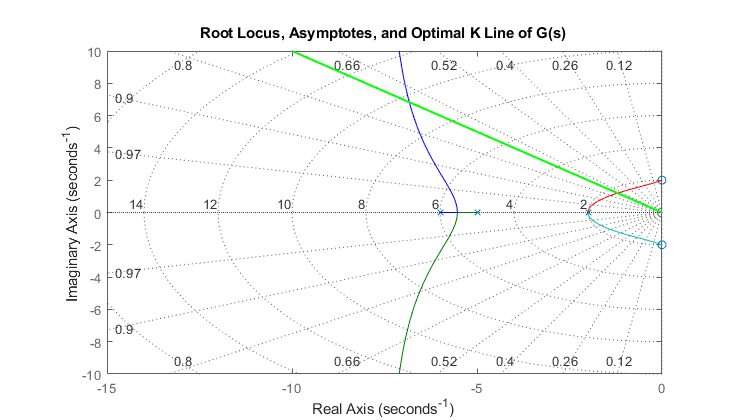
\includegraphics[width=0.9\textwidth]{7-16B.png}
\begin{lstlisting}
% Define the numerator and denominator of the transfer function G(s)
numerator = [1 0 4];
denominator = conv([1 2], conv([1 2], conv([1 5], [1 6]))); % Convolution of the factors to get the denominator polynomial

% Create the transfer function in MATLAB
G_s = tf(numerator, denominator);

% Plot the root locus
figure;
rlocus(G_s);
hold on;

% Asymptote information from earlier analysis
asymptote_angles = [90, 270]; % Degrees
asymptote_real_intercept = -7.5; % Real axis intercept

% Plot the asymptotes
for k = 1:length(asymptote_angles)
    % Convert angle to radians for MATLAB functions
    angle_rad = deg2rad(asymptote_angles(k));
    
    % These are very large numbers to ensure the lines go to the edge of the plot
    asymptote_x = asymptote_real_intercept : 0.1 : asymptote_real_intercept + 1000*cos(angle_rad);
    asymptote_y = 0 + (asymptote_x - asymptote_real_intercept)*tan(angle_rad);
    
    % Plot the asymptote
    plot(asymptote_x, asymptote_y, 'r--', 'LineWidth', 1.5); % Dashed red line
end

% Add the 135 degree line to find optimal K value
optimal_angle = 135; % Degrees
optimal_angle_rad = deg2rad(optimal_angle);

% Plot the 135 degree line
x_line = -10:0.1:0; % Change this range as needed
y_line = tan(optimal_angle_rad) * x_line;
plot(x_line, y_line, 'g-', 'LineWidth', 1.5); % Solid green line

% Set plot limits and labels
xlim([-15, 0]);
ylim([-10, 10]);
xlabel('Real Axis');
ylabel('Imaginary Axis');
title('Root Locus, Asymptotes, and Optimal K Line of G(s)');

% Add grid and hold off the plot
grid on;
hold off;

\end{lstlisting}



\end{document}
